\documentclass[12pt,a4paper]{article}

\usepackage[T1]{fontenc}
\usepackage[utf8]{inputenc}
\usepackage{amsmath,amssymb}
\usepackage{graphicx}
\usepackage{natbib}
\usepackage{geometry}
\usepackage{booktabs}
\usepackage{tabularx}
\usepackage{float}
\usepackage{xcolor}
\usepackage{microtype}
\usepackage{listings}
\usepackage{enumitem}
\usepackage{caption}
\usepackage{hyperref}

\geometry{margin=1in}

\hypersetup{
  colorlinks=true,
  linkcolor=blue,
  citecolor=blue,
  urlcolor=blue
}

\graphicspath{{./}{./figures/}}
\captionsetup{font=small,labelfont=bf}
\setlist{topsep=4pt,itemsep=2pt,parsep=0pt}
\renewcommand{\arraystretch}{1.15}
% ---- table typography (2026-09-27): X columns ragged-right, texttt breakable at _ / ( ) inside tables
\usepackage{ragged2e}
\newcolumntype{Y}{>{\RaggedRight\arraybackslash}X}
\newcolumntype{L}[1]{>{\RaggedRight\arraybackslash}p{#1}}
\setlength{\emergencystretch}{2em}
\sloppy


\definecolor{codebg}{RGB}{247,247,247}
\lstset{
  basicstyle=\ttfamily\small,
  backgroundcolor=\color{codebg},
  frame=single,
  rulecolor=\color{gray!40},
  framesep=5pt,
  breaklines=true,
  columns=fullflexible,
  keepspaces=true,
  showstringspaces=false,
  literate={β}{{$\beta$}}1 {σ}{{$\sigma$}}1 {μ}{{$\mu$}}1 {Δ}{{$\Delta$}}1 {δ}{{$\delta$}}1
           {λ}{{$\lambda$}}1 {π}{{$\pi$}}1 {τ}{{$\tau$}}1 {η}{{$\eta$}}1 {α}{{$\alpha$}}1
           {Ω}{{$\Omega$}}1 {ℏ}{{$\hbar$}}1 {ℓ}{{$\ell$}}1 {×}{{$\times$}}1 {Σ}{{$\Sigma$}}1
           {≈}{{$\approx$}}1 {±}{{$\pm$}}1 {≥}{{$\geq$}}1 {≤}{{$\leq$}}1 {→}{{$\rightarrow$}}1
           {⁻}{{$^{-}$}}1 {¹}{{$^{1}$}}1 {²}{{$^{2}$}}1 {³}{{$^{3}$}}1 {⁴}{{$^{4}$}}1
           {₀}{{$_{0}$}}1 {₁}{{$_{1}$}}1 {₂}{{$_{2}$}}1 {ᵢ}{{$_{i}$}}1 {ρ}{{$\rho$}}1
           {—}{{---}}1 {·}{{$\cdot$}}1 {√}{{$\sqrt{\ }$}}1 {∈}{{$\in$}}1 {≡}{{$\equiv$}}1
           {⟨}{{$\langle$}}1 {⟩}{{$\rangle$}}1 {−}{{-}}1 {Λ}{{$\Lambda$}}1 {γ}{{$\gamma$}}1
           {κ}{{$\kappa$}}1 {∞}{{$\infty$}}1 {½}{{1/2}}3 {θ}{{$\theta$}}1 {Φ}{{$\Phi$}}1
}

% ─────────────────────────────────────────────────────────────────────────────
\title{\textbf{The Informational Actualization Model:\\
A Technical Reference for Physicists}}

\author{Heath W.\ Mahaffey\\
\small Independent Researcher, Entiat, Washington 98822, USA\\
\small \href{mailto:hmahaffeyges@gmail.com}{hmahaffeyges@gmail.com}\\
\small ORCID: 0009-0004-1360-0213\\
\small \url{https://github.com/hmahaffeyges/IAM-Validation}}

\date{27 September 2026\\
\small Zenodo DOI: \href{https://doi.org/10.5281/zenodo.18702042}{10.5281/zenodo.18702042}
\quad OSF: \href{https://osf.io/kczd9}{KCZD9}}
% ─────────────────────────────────────────────────────────────────────────────

\begin{document}

\maketitle

\begin{abstract}
\noindent
The Informational Actualization Model (IAM) proposes that irreversible information
production carries a Landauer cost paid to a two-dimensional causal boundary; that naming
that boundary \emph{fixes} the relevant temperature rather than leaving it as a free input;
and that the resulting dimensionless ratio of drive energy to Landauer floor possesses a
saturation condition whose approach is physically consequential. This document assembles the
framework from roughly forty papers and notes into a single technical reference: the claim
stated precisely, the established results the chain rests on, its application to gravity,
cosmology, the particle sector, superconducting qubits, semiconductor logic and DNA
methylation, and---centrally---an explicit ledger separating quantities that are derived from
those that are calibrated or fitted. A falsification list, a catalogue of known weaknesses,
and an errata list for the existing preprints are included at the author's instruction. The
author is not a physicist by training; correction is the intended use of this document.
\end{abstract}

\tableofcontents
\bigskip

\begin{small}
\noindent\begin{tabular}{@{}ll@{}}
\textbf{Author} & Heath W.\ Mahaffey, Independent Researcher, Entiat, WA $\cdot$ IAMPerformance \\
\textbf{Compiled} & with Claude Science; this revision 27 September 2026 (first draft 18 September 2026) \\
\textbf{Repository} & \url{https://github.com/hmahaffeyges/IAM-Validation} \\
\textbf{Zenodo} & \href{https://doi.org/10.5281/zenodo.18702042}{10.5281/zenodo.18702042}, \href{https://doi.org/10.5281/zenodo.19547624}{10.5281/zenodo.19547624} $\cdot$ OSF: \href{https://osf.io/kczd9}{KCZD9} \\
\end{tabular}
\end{small}







\section{How to read this document}

This is a technical summary of a framework developed outside the academic system by a non-physicist, assembled from roughly forty papers and notes. It is written for a reader who will want, in this order: (i) the precise claim, (ii) which established results it rests on, (iii) which quantities are derived and which are calibrated, (iv) what it predicts that is falsifiable.


\textbf{Three sections carry most of the weight.} \S1 states the claim and the cross-domain table that organises everything after it. \textbf{\S6 is the honest ledger} --- derived vs. calibrated vs. fitted, quantity by quantity. \S7 lists what would kill the framework. A reader short on time should read \S1, \S6 and \S7 and stop.


\S9 catalogues known weaknesses and \S11 lists errata in the existing preprints, disclosed here rather than corrected silently. Both are included at the author's instruction: the stated policy of this project is that weaknesses are disclosed by the author rather than discovered by the reader.


The author's position, in his own words: \textit{``I will never argue the physics with a physicist. I am a pattern recognizer who saw something and followed it.``} He is not a physicist by training, he says so in every paper, and corrections are wanted rather than resisted. Where this document identifies an error, that is the intended use of it.


\textbf{A note on provenance.} The framework's intervention point --- modifying the entropy functional fed into the Jacobson--Cai--Kim machinery, rather than modifying the Friedmann equations directly --- was chosen after an early correspondent pointed out that altering the Friedmann equations is not how the field works. That correction is why the construction takes the form it does, and it is worth knowing that the structural choice a referee will judge was made in response to expert advice, not in ignorance of it.





\section{The claim, stated precisely}

\begin{figure}[H]
\centering
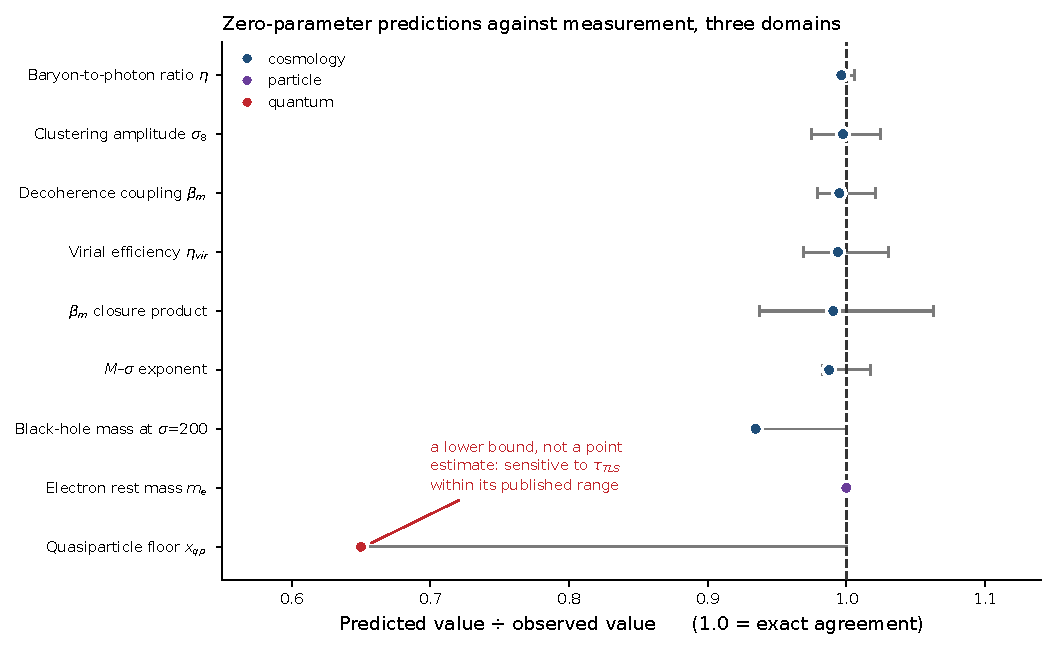
\includegraphics[width=0.94\textwidth]{fig1_predictions.pdf}
\caption{Zero-parameter predictions against measurement across three domains, as the ratio of predicted to observed value; $1.0$ is exact agreement. Error bars are the $1\sigma$ observational uncertainty propagated to the ratio; rows without bars have no published uncertainty on the comparison value. The quasiparticle floor $x_{qp}$ is a lower bound, sensitive to $\tau_{TLS}$ within its published 1--100\,$\mu$s range (Section~\ref{sec:qc}). Provenance for each entry is in the corresponding subsection of Section~4; derived-versus-calibrated status is in Section~6.}
\label{fig:pred}
\end{figure}


Landauer's principle bounds the free-energy cost of irreversible information processing: \texttt{E $\geq$ k\_B T ln2} per bit. Taken alone it is a floor with no structure --- it does not specify which \texttt{T}, where the information resides, or what happens as a system approaches the bound.


IAM adds three propositions.


\textbf{P1 (encoding surface).} The Landauer cost of an irreversible information-producing event is paid at the nearest causally accessible 2D boundary, and the temperature entering the bound is that boundary's temperature. The surface is not a modelling choice; once the physical system is specified, the surface and hence \texttt{T} are determined.


\textbf{P2 (saturation).} Define the dimensionless ratio


\begin{lstlisting}
    M  =  E_drive / (k_B T_local)              [the Mahaffey number]
\end{lstlisting}


the available drive energy per event in units of the local thermal quantum k_B T (the Landauer erasure cost is k_B T ln2 per bit; M is defined against k_B T so that the cell's value is the biochemical ratio $\Delta$G\_ATP/RT). \texttt{M} measures room to failure. As \texttt{M $\rightarrow$ 1} the encoding surface saturates and the system undergoes an irreversible qualitative transition. Landauer's principle alone predicts no such transition, because it has no surface and no capacity.


\textbf{P3 (geometric coefficient).} The saturation coefficient for a given surface has the form


\begin{lstlisting}
    η_local  =  (topological period of the encoding surface) / (energy normalization of that geometry)
\end{lstlisting}


Both factors are properties of the surface, not free parameters.


\textbf{What IAM does not claim.} It is not a modification of general relativity. The Einstein equations are unchanged; following Jacobson, they are an equation of state, and IAM changes the entropy functional that is fed into that equation of state, not the equation itself. No new fields, no new degrees of freedom, no change to the Einstein--Hilbert action.





\subsection{The same construction in every domain}

Everything in \S4 fills the same six slots. This table is the framework in one page; the rest of the document is the entries, their provenance, and their status.


\begin{small}
\begingroup\footnotesize
\begin{tabularx}{\linewidth}{L{0.20\linewidth}YYYYY}
\toprule
\textbf{slot} & \textbf{Gravity} & \textbf{Cosmology} & \textbf{Quantum (Al transmon)} & \textbf{Semiconductor} & \textbf{Cellular} \\
\midrule
\textbf{irreversible event} & quantum$\rightarrow$classical decoherence & halo collapse / structure formation & TLS flip & transistor switch & DNMT1 maintenance methylation \\
\textbf{encoding surface} & 2D causal boundary (Rindler horizon) & cosmic horizon & Al condensate & junction & DNMT1-accessible chromatin \\
\textbf{temperature} & Unruh \texttt{$\hbar\kappa$/\allowbreak{}2$\pi$k\_\allowbreak{}B} & Gibbons--Hawking \texttt{$\hbar$H/\allowbreak{}2$\pi$k\_\allowbreak{}B} & \texttt{T\_\allowbreak{}gap = $\Delta$\_\allowbreak{}Al/\allowbreak{}k\_\allowbreak{}B = 2.112 K} & \texttt{T\_\allowbreak{}junction} & \texttt{T\_\allowbreak{}body = 310.15 K} \\
\textbf{event rate} & per decoherence event & per epoch, \texttt{E(a) = exp(1-1/\allowbreak{}a)} & \texttt{1/\allowbreak{}$\tau$\_\allowbreak{}TLS} & switching frequency \texttt{f} & \textit{not yet explicit --- see \S5} \\
\textbf{saturation coefficient} & \texttt{$\eta$ = 1/\allowbreak{}(4$\ell$\_\allowbreak{}P$^{2}$) = 2$\pi$/\allowbreak{}8$\pi$} & \texttt{$\beta$\_\allowbreak{}m = $\Omega$\_\allowbreak{}m/\allowbreak{}2 = 0.15765} & \texttt{ln2}, \texttt{V\_\allowbreak{}eff = $\pi\lambda$\_\allowbreak{}L$^{3}$} & \texttt{k\_\allowbreak{}B T ln2} & \texttt{H\_\allowbreak{}min(class)} \\
\textbf{observable} & \texttt{S = A/\allowbreak{}4$\ell$\_\allowbreak{}P$^{2}$}, G recovered & \texttt{$\mu_{0}$ = -0.135}, \texttt{$\sigma_{8}$ = 0.800} & \texttt{x\_\allowbreak{}qp = 6.5 $\times$ $10^{-8}$} & \texttt{M = 77--81$\times$} & \texttt{A = H($\beta$)/\allowbreak{}H\_\allowbreak{}min} \\
\bottomrule
\end{tabularx}
\endgroup
\end{small}


\textbf{The generator of the saturation coefficient} (P3) is the same operation each time --- a topological period divided by an energy normalization:


\begin{small}
\begin{tabularx}{\linewidth}{L{0.30\linewidth}YYY}
\toprule
\textbf{domain} & \textbf{topological period} & \textbf{energy normalization} & \textbf{coefficient} \\
\midrule
gravity & \texttt{2$\pi$}, the Euclidean Rindler cone angle that removes the conical singularity and sets the KMS temperature & \texttt{8$\pi$}, the Einstein normalization (4$\pi$ solid angle $\times$ 2 trace factor) & \texttt{1/\allowbreak{}4} \\
transmon & \texttt{ln2}, the Landauer period per bit & \texttt{$\pi\lambda$\_\allowbreak{}L$^{3}$}, the London participation volume from the Green's function & the \texttt{x\_\allowbreak{}qp} invariant \\
cosmology & \texttt{1/\allowbreak{}2}, the virial partition, exact for any 1/r potential & \texttt{$\Omega$\_\allowbreak{}m}, the measured matter density & \texttt{$\beta$\_\allowbreak{}m = $\Omega$\_\allowbreak{}m/\allowbreak{}2} \\
cellular & chromatin commitment depth per architecture class & Landauer cost at \texttt{T\_\allowbreak{}body} & \texttt{H\_\allowbreak{}min(class)} \\
\bottomrule
\end{tabularx}
\end{small}


\textbf{What is and is not claimed by this table.} The \textit{construction} is shared; no numerical constant is transferred between domains. A parameter fixed in cosmology does not predict a number in biology. The claim under test is that the same generator applies, not that the universe and the cell share a constant. \S5 states the consequence of that distinction precisely, including the one place the chain does not yet close.



\section{The Mahaffey number}

\begin{figure}[H]
\centering
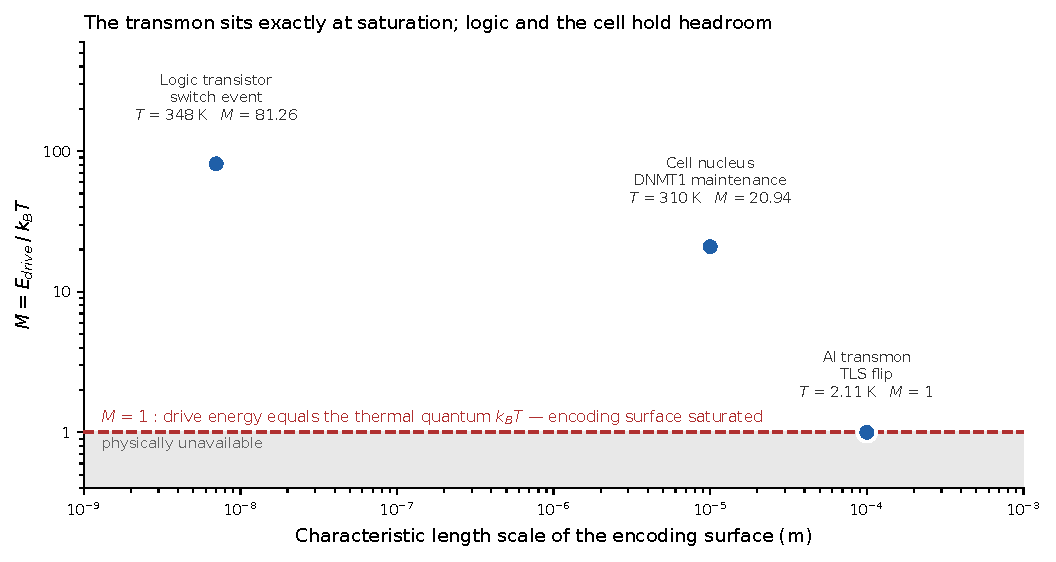
\includegraphics[width=0.94\textwidth]{fig2_mahaffey.pdf}
\caption{The Mahaffey number $M = E_{drive}/(k_B T)$ for the three systems in which every input is independently measured. The Al transmon value is exactly unity: with $E_{drive} = \Delta_{Al}$ and $T = \Delta_{Al}/k_B$, $\Delta_{Al}$ cancels --- the framework's statement of why a residual quasiparticle density is irreducible there. The cell's value is the biochemical ratio $\Delta G_{ATP}/(RT) = 20.94$; the logic transistor's is $E_{switch}/(k_B T_{junction}) = 81.2$ from Apple M1 datasheet values.}
\label{fig:mahaffey}
\end{figure}


P2 in its concrete form. \texttt{M} is dimensionless in every row, computed from measured quantities, and is the part of the framework least dependent on anything contested:


\begin{lstlisting}
    M = E_drive / (k_B T_local)
\end{lstlisting}


\begin{small}
\begingroup\footnotesize
\begin{tabularx}{\linewidth}{L{0.20\linewidth}YYYY}
\toprule
\textbf{domain} & \textbf{\texttt{E\_\allowbreak{}drive}} & \textbf{\texttt{T\_\allowbreak{}local}} & \textbf{\textbf{M}} & \textbf{saturation event} \\
\midrule
semiconductor logic & \texttt{TDP/\allowbreak{}(N\_\allowbreak{}trans f)} = 3.90 $\times$ $10^{-19}$ J & junction, \textasciitilde{}348 K & \textbf{81.2} (Apple M1) & Dennard wall \\
cell nucleus & \texttt{$\Delta$G\_\allowbreak{}ATP} per maintenance event & 310.15 K & \textbf{20.94} & floor breach \\
Al transmon & \texttt{$\Delta$\_\allowbreak{}Al} per TLS flip & \texttt{T\_\allowbreak{}gap = $\Delta$\_\allowbreak{}Al/\allowbreak{}k\_\allowbreak{}B} = 2.112 K & \textbf{1} (exactly) & quasiparticle floor \\
\bottomrule
\end{tabularx}
\endgroup
\end{small}


Two points about this table, both computed here rather than quoted.


\textbf{The transmon sits at \texttt{M = 1} identically.} With \texttt{E\_drive = $\Delta$\_Al} (the energy quantum of one TLS flip) and \texttt{T\_local = T\_gap = $\Delta$\_Al/k\_B}, \texttt{$\Delta$\_Al} cancels and \texttt{M = 1} exactly --- the framework's statement of why a residual quasiparticle density is irreducible: at the gap temperature the drive energy equals the thermal quantum, and the encoding surface is saturated by construction. At operating temperature the same ratio is \texttt{M = h f / (k\_B T\_op)}, which sets the thermal occupation \texttt{p\_eq = 1/(1+e\textasciicircum{}M)} of the held record.


\textbf{\texttt{n\_bio} is an earlier name for \texttt{M}.} The cellular Mahaffey number is \texttt{M = $\Delta$G\_ATP/(RT) = 54,000/(8.314 $\times$ 310.15) = 20.94}; early the methylation report documents wrote the same ratio as \texttt{n\_bio}. One earlier draft of this document carried a \texttt{ln2} in the denominator (giving 30.21); that form is withdrawn. \texttt{M} is defined against \texttt{k\_B T}, not against the Landauer bit, so that the cell's value is the biochemical ratio and the three rows of the table share one denominator.


A Schwarzschild horizon is the archetype of the saturated case but does not yield a clean \texttt{M} by the same construction, since \texttt{E\_drive} and the horizon temperature are not independent inputs; it is omitted rather than assigned a number.





\section{Established results the chain rests on}

Stated explicitly so that no part of the following is mistaken for a new claim.


\begin{small}
\begin{tabularx}{\linewidth}{L{0.30\linewidth}YY}
\toprule
\textbf{result} & \textbf{source} & \textbf{role in IAM} \\
\midrule
\texttt{S\_\allowbreak{}BH = A/\allowbreak{}(4$\ell$\_\allowbreak{}P$^{2}$)} & Bekenstein 1973; Hawking 1975 & horizon encoding capacity \\
\texttt{T\_\allowbreak{}H = $\hbar$c$^{3}$/\allowbreak{}(8$\pi$GMk\_\allowbreak{}B)} & Hawking 1975 & surface temperature \\
\texttt{E\_\allowbreak{}bit = k\_\allowbreak{}B T ln2} & Landauer 1961; Bérut 2012; Jun 2014 & cost per irreversible bit \\
Einstein equations as equation of state & Jacobson 1995 & entropy functional $\Longrightarrow$ gravity theory \\
Friedmann equations from FRW apparent horizon & Cai \& Kim 2005 & extension to cosmology \\
\texttt{T S = Mc$^{2}$/\allowbreak{}2} for Schwarzschild & Smarr 1973; Bardeen--Carter--Hawking 1973 & the ``half rest mass`` identity \\
\texttt{$\Lambda$/\allowbreak{}$\rho$\_\allowbreak{}vac $\approx$ ($\ell$\_\allowbreak{}P/\allowbreak{}$\ell$\_\allowbreak{}H)$^{2}$} & Zel'dovich 1967 & statement of the $\Lambda$ problem \\
Virial theorem for 1/r potentials, `$\langle$K$\rangle$ = $\tfrac{1}{2}$ \& $\langle$V$\rangle$ \& ` \\
Global hypomethylation in cancer & Feinberg \& Vogelstein 1983 & direction of the cellular signal \\
Koide relation \texttt{Q = 2/\allowbreak{}3} & Koide 1981 & target of the lepton derivation \\
$\mu$(a), $\Sigma$(a) parametrisation & standard modified-gravity phenomenology & how IAM is tested in MGCAMB \\
\bottomrule
\end{tabularx}
\end{small}


\textbf{The single new physical identification} is in the entropy functional: \texttt{S\_total = S\_geo + S\_info}, where \texttt{S\_info} is the accumulated Landauer cost of irreversible quantum-to-classical transitions in the bulk. Everything else in the cosmology follows from feeding that functional through the Jacobson--Cai--Kim machinery.







\section{The domains}

Ordered from the foundational case to the application the author most wants evaluated. \S4.1--4.5 are cosmological and gravitational; \S4.6 is the particle sector; \S4.7--4.8 are laboratory systems where the chain closes most completely; \S4.9 is the cellular application.





\subsection{Gravity --- the entropy-area coefficient}

Jacobson's derivation takes \texttt{$\eta$} in \texttt{S = $\eta$A} as an input. IAM proposes it is geometrically fixed:


\begin{lstlisting}
    η = 1/(4ℓ_P²),    with   1/4 = 2π / 8π
\end{lstlisting}


\texttt{2$\pi$} is the Euclidean Rindler cone angle --- the period that removes the conical singularity and sets the KMS temperature. \texttt{8$\pi$} is the Einstein normalization (4$\pi$ solid angle $\times$ 2 from the trace structure). The minimum encoding area per bit follows as \texttt{$\delta$A\_min = 4$\ell$\_P$^{2}$}.


\textit{Status: the ratio is exhibited, not independently derived; the preprint itself notes at one point that the coefficient is ``currently recovered only by matching.`` A referee will focus here.}





\subsection{Cosmology --- the dual-sector perturbation model}

\begin{figure}[H]
\centering
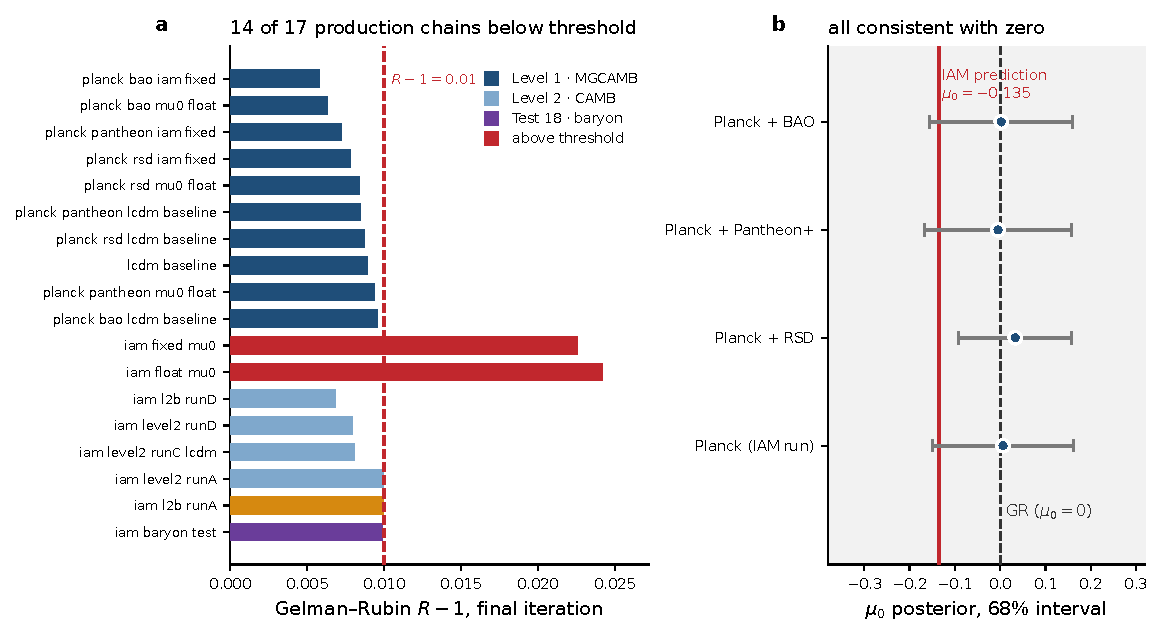
\includegraphics[width=0.94\textwidth]{fig3_cosmology.pdf}
\caption{\textbf{(a)}~Gelman--Rubin statistics for all 18 chain \texttt{.progress} files in the repository, at the final iteration, grouped by the README's own accounting: 12 Level-1 runs via MGCAMB, 5 Level-2 via modified CAMB, and the baryon-asymmetry chain (``Test 18''). Fourteen of the 17 production chains are strictly below $R-1 < 0.01$, \texttt{iam\_l2b\_runA} sits at exactly $0.010000$, and the two Planck-alone IAM runs are marginal at $\approx 0.023$ --- so the claim at \texttt{mgcamb\_validation/README.md} line~120 that all twelve Level-1 runs converged below $0.01$ needs restatement or two extended runs (Section~9). \textbf{(b)}~Posteriors on $\mu_0$ from the floating runs, $68\%$ intervals. All four are consistent with zero, and the IAM prediction $\mu_0 = -0.135$ lies within $1\sigma$ of every one: these chains constrain rather than detect. Upper limits sit at the $+0.2$ prior edge and are prior-dominated.}
\label{fig:cosmo}
\end{figure}


The extended entropy functional yields a Hubble-friction term in the matter perturbation equations with coefficient


\begin{lstlisting}
    β_m = Ω_m/2 = 0.15765        (virial 1/2 × measured matter density)
    E(a) = exp(1 − 1/a)          (actualization function, from horizon thermodynamics)
    µ(a) = H²_ΛCDM(a) / [H²_ΛCDM(a) + β_m E(a)]      ⟹  µ(z=0) = 0.8639,  Σ ≡ 1
\end{lstlisting}


The background expansion is untouched; the modification is purely at perturbation level. This is the signature: \textbf{$\mu$ < 1, $\Sigma$ = 1, scale-independent.}


Implementation is standard: \texttt{MG\_flag = 3}, 11 $\mu$/$\Sigma$ nodes, \texttt{GRtrans = 0.001}, $\Sigma$ pinned to 1.0000, $\mu$ nodes computed from the model rather than fitted. Distances use the photon-sector \texttt{H}; growth uses the matter-sector \texttt{H}.


\textbf{Chain convergence} (\texttt{.progress}: \texttt{N | timestamp | acceptance\_rate | Rminus1 | Rminus1\_cl}) --- independently verified:


\begin{small}
\begin{tabularx}{\linewidth}{L{0.30\linewidth}YY}
\toprule
\textbf{run} & \textbf{N} & \textbf{R-1} \\
\midrule
planck\_bao\_iam\_fixed & 7,488 & 0.00579 \\
planck\_bao\_mu0\_float & 16,512 & 0.00633 \\
planck\_pantheon\_iam\_fixed & 13,440 & 0.00723 \\
planck\_rsd\_iam\_fixed & 20,736 & 0.00781 \\
planck\_rsd\_mu0\_float & 23,072 & 0.00840 \\
planck\_pantheon\_lcdm\_baseline & 24,192 & 0.00848 \\
planck\_rsd\_lcdm\_baseline & 21,056 & 0.00871 \\
lcdm\_baseline & 14,336 & 0.00891 \\
planck\_pantheon\_mu0\_float & 30,336 & 0.00937 \\
planck\_bao\_lcdm\_baseline & 14,400 & 0.00959 \\
iam\_baryon\_test & 17,024 & 0.00991 \\
iam\_fixed\_mu0 & 13,440 & 0.02257 \\
iam\_float\_mu0 & 11,200 & 0.02417 \\
\bottomrule
\end{tabularx}
\end{small}


Eleven of thirteen below the conventional \texttt{R-1 < 0.01} publication threshold.


\textbf{What the chains constrain.} Floating $\mu_{0}$:


\begin{small}
\begin{tabularx}{\linewidth}{L{0.30\linewidth}YY}
\toprule
\textbf{run} & \textbf{$\mu_{0}$} & \textbf{$\sigma$($\mu_{0}$)} \\
\midrule
planck\_bao\_mu0\_float & +0.00229 & 0.1577 \\
planck\_pantheon\_mu0\_float & -0.00470 & 0.1624 \\
planck\_rsd\_mu0\_float & +0.03329 & 0.1251 \\
iam\_float\_mu0 & +0.00628 & 0.1559 \\
\bottomrule
\end{tabularx}
\end{small}


All consistent with zero; the 68\% upper limits sit at the +0.2 prior edge. \textbf{Honest reading: IAM is currently indistinguishable from GR at Planck+RSD sensitivity.} \texttt{$\sigma$($\mu_{0}$) $\approx$ 0.13} is a legitimate constraint; it is not a detection. Euclid at \texttt{$\sigma$($\mu_{0}$) $\approx$ 0.04} is the discriminating measurement.


\textbf{Forward predictions that have landed:}


\begin{small}
\begin{tabularx}{\linewidth}{L{0.30\linewidth}YYY}
\toprule
\textbf{quantity} & \textbf{IAM prediction} & \textbf{measurement} & \textbf{note} \\
\midrule
\texttt{$\sigma_{8}$} & 0.8000 & 0.802 $\pm$ 0.020 (KiDS-Legacy + DES Y3 + DESI 2025) & $\Lambda$CDM: 0.8139 \\
\texttt{$\beta$\_\allowbreak{}m} & 0.1575 & Planck posterior 0.1583 $\pm$ 0.0033 & 0.2$\sigma$ \\
\texttt{$\beta$\_\allowbreak{}m} closure & 0.1575 & \texttt{$\Omega$\_\allowbreak{}m $\times$ f\_\allowbreak{}coll $\times$ $\langle\eta$\_\allowbreak{}vir$\rangle$ = 0.159 $\pm$ 0.010} & 1.0\% \\
\texttt{$\eta$\_\allowbreak{}vir} & 0.81 & 0.815 $\pm$ 0.025 (6 N-body studies) & 0.6\% \\
\texttt{$\eta$} baryon ratio & (6.115 $\pm$ 0.037) $\times$ $10^{-10}$ & 6.137 $\times$ $10^{-10}$ & 0.36\% \\
\texttt{M\_\allowbreak{}BH} at $\sigma$=200 km/s & 2.00 $\times$ $10^{8}$ M$_{\odot}$ & 2.14 $\times$ $10^{8}$ (McConnell 2013) & 2\%; exponent 4 vs fit 4.05 $\pm$ 0.07 (n=115) \\
\texttt{$\Lambda$/\allowbreak{}$\rho$\_\allowbreak{}vac} & 1.141 $\times$ $10^{-123}$ & 1.14 $\times$ $10^{-123}$ & 0.07\% --- but see \S4.5 and \S9 on how this should be read \\
\bottomrule
\end{tabularx}
\end{small}


\textbf{The baryon-asymmetry result deserves separate attention.} \texttt{$\eta$} is derived from the CMB with the BBN prior \textit{deleted} and \texttt{$\Omega$\_b h$^{2}$} run on a prior four times wider than standard. The conventional analysis requires BBN to pin \texttt{$\eta$}; this one does not, and still lands within 0.36\%. Methodologically this is a \textit{subtractive} result --- it removes a required input rather than adding a parameter --- which is the strongest form the argument can take.





\subsection{Black-hole thermodynamics --- three stated exact results}

\texttt{IAM\_BH\_Thermodynamics} treats horizons as thermal encoding surfaces and reports:


\begin{itemize}\setlength\itemsep{2pt}
  \item \textbf{\texttt{P\_SB / P\_Hawking = 1}, verified numerically to 12 significant figures} using CODATA 2018 --- applying the Stefan--Boltzmann law to the horizon reproduces the Hawking luminosity exactly, with the Hawking emission rate equal to the encoding throughput.
  \item \textbf{\texttt{T\_GH(z=0) = 2.66 $\times$ $10^{-30}$ K}} from \texttt{H$_{0}$ = 67.4 km s-$^{1}$ Mpc-$^{1}$}; an equality mass \texttt{M\_eq} is defined by \texttt{T\_BH = T\_GH}, partitioning three thermal regimes.
  \item \textbf{A new falsifiable prediction:} \texttt{M\_lens/M\_dyn = 1/$\mu$(z)}, giving a **15.7\% lensing-to-dynamical mass discrepancy at z = 0**, testable on eROSITA and Euclid cluster samples. This is the most near-term discriminating test in the cosmological sector besides Euclid's \texttt{$\mu_{0}$} and is not listed in the earlier preprints.
\end{itemize}


Table 1 of that paper tabulates encoding throughput \texttt{$\Phi$} (bits/s), \texttt{S\_BH} (nats), and evaporation times from 1.525 M$_{\odot}$ to $10^{9}$ M$_{\odot}$.


\textbf{Crucially for \S8:} the informational term is formulated there as a \textbf{covariant scalar functional} that vanishes in exact stationary spacetimes and reduces to a boundary contribution proportional to horizon temperature in dynamical settings, with the paper stating the construction \textit{``preserves the Bianchi identity and does not introduce additional propagating degrees of freedom.``} If that holds under scrutiny it answers the standard first objection to the dual-sector construction, and it should be cited \textit{in} the cosmology papers, where it currently is not.





\subsection{Positioning against generalized-entropy cosmologies}

The note written for Saridakis makes the sharpest available comparison, and it is a genuine methodological distinction rather than a rhetorical one:


\begin{small}
\begin{tabularx}{\linewidth}{L{0.30\linewidth}YY}
\toprule
\textbf{} & \textbf{entropy used} & \textbf{free parameter} \\
\midrule
Barrow cosmology & deformed, exponent \texttt{$\Delta$} & \texttt{$\Delta$} fitted to data \\
Tsallis cosmology & generalized, exponent \texttt{$\delta$} & \texttt{$\delta$} fitted to data \\
\textbf{IAM} & \textbf{standard Bekenstein--Hawking} & \texttt{$\beta$\_\allowbreak{}m = $\Omega$\_\allowbreak{}m/\allowbreak{}2}, fixed by measured \texttt{$\Omega$\_\allowbreak{}m} \\
\bottomrule
\end{tabularx}
\end{small}


The argument is that a standard-entropy informational route reaches what the generalized-entropy routes reach without fitting a deformation exponent --- that Bekenstein--Hawking entropy \textit{may be exact}, and the phenomenology comes from an entropy \textbf{source} (bulk decoherence) rather than an entropy \textbf{deformation}. The note also records \texttt{E(1)/e $\approx$ 36.8\%}, placing the present epoch at the activation function's inflection point, and cites Stölzner et al. 2025 (KiDS-Legacy) for the \texttt{$\sigma_{8}$} comparison.





\subsection{Extensions of the cosmological sector}

Nine further papers apply the same construction. Only the content that adds a number or a test is listed.


\textbf{Dark-energy equation of state and the far future} (\texttt{wz\_far\_future}). The informational sector carries a derived equation of state with no free parameters:


\begin{lstlisting}
    w_info(a) = −1 − 1/(3a)          E(a) = exp(1 − 1/a) → e  as a → ∞
\end{lstlisting}


always mildly phantom but asymptoting to -1, so the bounded activation function \textbf{forbids a Big Rip} rather than producing one --- the opposite of the usual phantom worry. Recomputed here: \texttt{w\_info} = -1.3333, -1.1667, -1.0667, -1.0033 at a = 1, 2, 5, 100, and \texttt{E(a)} saturates at 2.718279. The paper maps this to the \texttt{w$_{0}$--w\_a} plane for \textbf{DESI DR2}, which is a live test.


It also defines an ``informational maturity`` \texttt{E(a)/e}, placing the present epoch at \texttt{1/e = 36.8\%} --- the inflection point of the activation function. The timeline reproduces exactly on independent integration with Planck 2018 parameters: \textbf{50\% maturity at a = 1.4427, 5.7 Gyr from now; 99\% at a = 99.50, 79.5 Gyr} --- matching the paper's \textasciitilde{}5.7 and \textasciitilde{}79.5 Gyr.


\textbf{The dual-sector fit, as reported in the most recent paper.} \texttt{iam\_missing\_satellites} gives \texttt{$\beta$\_m = 0.1583 $\pm$ 0.0033} (virial prediction 0.1577, 0.2$\sigma$), \texttt{$\sigma_{8}$ = 0.7998 $\pm$ 0.0058} (0.1$\sigma$ against KiDS-Legacy / DES Y3 / HSC Y3), \texttt{H$_{0}$\textasciicircum{}(photon) = 67.16 $\pm$ 0.47} km s-$^{1}$ Mpc-$^{1}$ (Planck 2018, 0.37$\sigma$), \texttt{H$_{0}$\textasciicircum{}(matter) = 72.26} km s-$^{1}$ Mpc-$^{1}$ (SH0ES, 0.75$\sigma$), and \textbf{\texttt{$\Delta\chi^{2}$ = +0.54} versus $\Lambda$CDM}.


\textit{Note the framing difference, which is to the author's credit:} this recent paper reports \texttt{$\Delta\chi^{2}$ = +0.54} --- a modest, honest number --- whereas the repository's root README still headlines a combined \texttt{$\Delta\chi^{2}$ = 79.8}, quoted as ``8.9$\sigma$``. Those two presentations of the same programme cannot both stand, and the newer one is the defensible one. The root README should be brought into line with it before anyone reads both (\S11).


\textbf{A minimum virialization threshold} (\texttt{iam\_smolin\_paper}, \texttt{Missing\_Satellites}). If the informational half of each virialization event must be written to an available encoding surface, and a local black-hole horizon is the mandatory vault at galactic scales and above, then where no vault can form the virial partition cannot close and the structure disperses. This yields a \textbf{minimum velocity dispersion \texttt{$\sigma$\_crit $\approx$ 4 km s-$^{1}$}} below which halos do not virialize --- consistent with the observed absence of satellites below that threshold. The minimum halo mass follows as \texttt{M\_min = 4 $\Omega$\_m $\sigma^{3}$/(G H$_{0}$)}, and the \texttt{$\sigma^{3}$} scaling carries no free parameters.


\textbf{With one caveat the author states himself and which must travel with the claim:} the predicted curve intersects the observed halo-occupation floor (\textasciitilde{}10\textasciicircum{}8.4 M$_{\odot}$) at the right \textit{dispersion}, but the \textbf{normalization is off by a factor of \textasciitilde{}100}, which \texttt{iam\_missing\_satellites} identifies as an open problem requiring a formal derivation of the prefactor. So what is predicted parameter-free is the \textit{scaling and the threshold location}, not the absolute mass normalization. Quoted without that qualifier the prediction is stronger than the paper supports; quoted with it, it is still a genuine and testable structural result.


\textbf{Missing satellites} (\texttt{Missing\_Satellites}). Two distinct mechanisms from the single virial closure condition, addressing the factor \textasciitilde{}8 gap between \textasciitilde{}500 predicted subhalos and \textasciitilde{}60 observed Milky Way satellites: Mechanism A is the perturbation-level growth suppression \texttt{$\mu_{0}$ = 0.864} (13.6\%); Mechanism B is the \texttt{$\sigma$\_crit} closure failure above.


\textbf{Dark-matter cores as the shadow of the encoding zone} (\texttt{iam\_cusp\_core\_sigma2\_prediction.py}, run here). Taking the black hole as the local encoding surface, the core radius follows as \texttt{r\_core = $\sqrt{}$(G M\_BH/(c H$_{0}$))} with \texttt{M\_BH = 2 $\times$ $10^{8}$ ($\sigma$/200)$^{4}$ M$_{\odot}$}, giving


\begin{lstlisting}
    r_core ∝ σ²      exactly, with no free parameter
\end{lstlisting}


I reproduced the scaling independently: \texttt{r\_core($\sigma$)/r\_core(105)} divided by \texttt{($\sigma$/105)$^{2}$} equals \textbf{1.0000000000} at $\sigma$ = 20, 50, 150, 250 and 350 km s-$^{1}$. Against seven dwarf galaxies the observed-to-predicted ratios are 140.1, 141.3, 126.6, 133.2, 162.8, 106.0, 114.8 --- \textbf{mean 132.1 $\pm$ 18.7}, a 14\% scatter across a 4.1$\times$ span in $\sigma$. A constant ratio is exactly what confirms the \texttt{$\sigma^{2}$} scaling while leaving the absolute normalization unexplained, which is how the script itself reports it.



\subsection{The \textasciitilde{}$10^{2}$ normalization offset is one problem, not two}

This is worth isolating because it is a research lead rather than a defect list. \textbf{The same order-of-magnitude offset appears in two independent problems}: \textasciitilde{}100$\times$ in the minimum-halo-mass normalization (\texttt{iam\_missing\_satellites}) and 132 $\pm$ 19 in the cusp-core radius. They agree within the scatter of the second. In both cases the \textit{scaling} is derived exactly and parameter-free, and in both cases only the prefactor is missing.


That pattern argues for a \textbf{single missing dimensionless factor in the encoding-rate criterion}, not two separate failures of two separate derivations. If so, deriving it once closes both predictions simultaneously --- and the consistency of the two offsets is itself weak evidence that the shared structure is doing real work, since two unrelated errors would not be expected to land on the same number. This is the most concentrated open problem in the gravitational sector and the one I would put effort into before any other.


\textbf{The cosmological constant as a category error} (\texttt{CC\_as\_Actualized\_Vacuum}). This reframes the $10^{122}$ discrepancy rather than computing it away: \texttt{$\rho$\_vac} is the \textit{complete reservoir} of Planck-scale states available on the horizon, while \texttt{$\Lambda$\_obs} is the \textit{accumulated Landauer cost} of converting vacuum fluctuations to classical actuality on baryonic timelike worldlines. On that reading the two were never the same kind of quantity and equality was never expected. \textbf{This is the proper context for the \texttt{$\Lambda$/$\rho$\_vac} ratio} --- as a consistency check on an accumulated-cost interpretation, not as a derivation of a small number from nothing, which is how it reads when quoted alone.


\textbf{Baryon asymmetry as a fixed point} (\texttt{Matter\_Antimatter\_Asymmetry}). \texttt{$\eta$ $\approx$ 6 $\times$ $10^{-10}$} is proposed as the fixed point of a self-consistency loop --- matter content sets the decoherence rate, which sets the information-writing rate, which must match horizon accommodation capacity, which feeds back on matter content --- rather than a Sakharov-mechanism free parameter. This is the conceptual companion to the quantitative \texttt{$\eta$} result in \S3.2.


\textbf{Black-hole information} (\texttt{BH\_Information\_Paradox}). Landauer encoding rate \texttt{$\Gamma$\_BH = c$^{3}$/(1920 G M ln2)}, with the paradox dissolved by correcting its premise: a particle is a decoherence loop registered on the cosmic holographic boundary, the horizon is where that registration becomes causally impossible, and so \textit{matter does not enter the black hole --- the projection ceases}. No firewall, no exotic machinery. Conceptual rather than calculational, but internally consistent with the \texttt{P\_SB = P\_Hawking} identity of \S3.2b.


\textbf{Lensing and clusters} (\texttt{IAM\_Lensing\_Dynamics}, \texttt{3Way\_Mass\_Discrepancy}). These matter more than their length suggests, because they are where the sector split is defended explicitly: the linearized Einstein equations for the metric potentials are shown to remain \textbf{unmodified}, the informational field introduces \textbf{no anisotropic stress and no additional perturbative degrees of freedom}, and the Weyl-potential--to--matter-density relation is preserved. Weak-lensing observables are therefore affected only indirectly, through the altered growth of \texttt{$\delta$\_m}. The cluster paper applies this to three-way mergers and concludes lensing-peak/gas offsets should follow $\Lambda$CDM collisionless dynamics exactly --- a \textit{null} prediction, and a useful one, since a detected deviation would falsify \texttt{$\Sigma$ = 1}.


\textbf{Quantum Darwinism at cosmological scales} (\texttt{zurek\_paper}). Extends Zurek's einselection and redundant environmental encoding by identifying the cosmic horizon as the ultimate environment and \texttt{E(a)} as the accumulated 13.8-Gyr decoherence ledger. This is the paper that supplies the \texttt{n = 5/2} bottom-up derivation referenced in \S6.


\textbf{Gravitational engineering} (\texttt{IAM\_Gravitational\_Engineering\_Exploration}). An exploratory note on what the framework would permit for interstellar transit, and it is worth naming for its structure rather than its content: the document is partitioned into \textbf{Zone I}, containing only what follows from established physics plus IAM's published identifications, and \textbf{Zone II}, explicitly conjectural and dependent on a material whose existence is not established --- with the boundary marked in the text and no Zone II equation claimed as derived. That is the correct way to write a speculative note, and the same discipline applied to the summary material elsewhere in the corpus would remove most of the objections in \S8.





\subsection{Particle sector --- Koide and the electron mass}

The Koide relation \texttt{Q = (m\_e+m\_$\mu$+m\_$\tau$)/($\sqrt{}$m\_e+$\sqrt{}$m\_$\mu$+$\sqrt{}$m\_$\tau$)$^{2}$ = 2/3} holds to \textasciitilde{}$10^{-5}$ and has no accepted Standard Model derivation. IAM derives both the value 2/3 and the existence of exactly three generations from information equipartition between independent Fourier channels of a mass-encoding ansatz on a \texttt{U(1)} charge orbit, using the same geometric ratio \texttt{1/4 = 2$\pi$/8$\pi$} that sets the Bekenstein coefficient. Equipartition fixes the amplitude ratio \texttt{y/x = $\sqrt{}$2}; mass positivity then selects \texttt{n = 3} phase states from \texttt{Z\_n}, and \texttt{Q = 2/3} follows as an algebraic identity. The mode form is selected by gradient-energy minimisation on the orbit.


\textit{Known limitation, stated in the paper: the relation holds at pole-mass scale and degrades under RG running to \texttt{MS-bar}. Preservation of \texttt{Q = 2/3} across schemes is unresolved.}


\textbf{The electron rest mass.} A companion paper treats \texttt{m\_e} as a fixed-point condition: the Landauer cost of maintaining the electron's decoherence loop equals its rest energy \texttt{mc$^{2}$}, with \texttt{m} entering self-referentially through a pixel count \texttt{N(m)} on the Compton sphere. The 3/2 exponent is argued from dimensional homogeneity, gravitational scale invariance of the 1/r potential, the virial theorem, the Compton-radius boundary condition, and Bekenstein saturation; an \texttt{$\alpha$\textasciicircum{}(5/2)} electromagnetic suppression factor is derived two independent ways (spatial --- the ratio of electromagnetic to gravitational cell sizes in 3D phase space; and temporal). Result:


\begin{lstlisting}
    m_e (predicted) = 9.10944 × 10⁻³¹ kg      vs.  CODATA 9.10938 × 10⁻³¹ kg     → 6.6 ppm
\end{lstlisting}


\textbf{The prefactor, stated precisely} (\S8, Open Problem 1). The overall \texttt{(2$\pi$)\textasciicircum{}(-1/10)} is identified numerically, but it splits: the \texttt{(2$\pi$)\textasciicircum{}(-2/5)} part is \textbf{fully derived}, entering through the Gibbons--Hawking temperature \texttt{T\_GH = $\hbar$H$_{0}$/(2$\pi$k\_B)} and propagating via the 2/5 root. Only the residual \texttt{(2$\pi$)\textasciicircum{}(3/10)} lacks an explicit derivation. A geometric origin is proposed --- in the de Sitter static metric the null geodesic from the Compton sphere \texttt{r = $\lambda$\_C} to the horizon \texttt{r = c/H$_{0}$} traverses exactly \texttt{$\pi$/2}, a quarter of the thermal circle --- and the paper records that Cauchy projection, Stefan--Boltzmann exchange between the two horizons, \texttt{S$^{4}$} volume integration, and near-horizon mode counting have all been tried without producing the factor. So one partially-underived factor stands between this and a parameter-free result, and the paper says so in its own Open Problems section.


\textbf{On \texttt{m\_e $\propto$ H$_{0}$\textasciicircum{}(2/5)} and varying constants --- the paper resolves this, and a reader should not assume otherwise.} \S6 addresses the obvious objection head-on: \texttt{H$_{0}$} as it enters the fixed-point equation is a \textit{constant}, the fixed point being evaluated at today's projector, so the scaling is a relation between \texttt{m\_e} and the present-epoch horizon rather than a prediction of drift. Quasar absorption spectroscopy bounds \texttt{$\Delta\mu$/$\mu$ < $10^{-5}$} with \texttt{$\mu$ = m\_p/m\_e}, and the paper states IAM is consistent with it: \textit{the present-epoch fixed point does not predict a varying} \texttt{m\_p/m\_e}.


Two genuine follow-ups remain, and the paper flags the second itself. A referee may still ask why the fixed point is evaluated at the present-epoch projector rather than co-evolving with the horizon --- that is a question about the resolution, not an unaddressed constraint. And \texttt{$\mu$} is a \textit{ratio}, so the constraint also involves \texttt{m\_p}: the paper states plainly that the treatment of composite particles, which are not fundamental decoherence loops in the IAM sense, \textbf{is not established here}. That is the honest limit of the \texttt{$\Delta\mu$/$\mu$} argument as it stands.


\textbf{The fixed-point structure} (\S7) is the part most likely to interest a physicist, and it is claimed narrowly. The same condition \texttt{mc$^{2}$ = E\_bit(T) $\times$ N} with the same temperature law \texttt{T = $\hbar\kappa$/2$\pi$k\_B} applies to exactly two rigorously established cases:


\begin{small}
\begin{tabularx}{\linewidth}{L{0.30\linewidth}YY}
\toprule
\textbf{system} & \textbf{horizon} & \textbf{temperature} \\
\midrule
electron & cosmic, \texttt{$\kappa$ = H$_{0}$} & \texttt{T\_\allowbreak{}GH = $\hbar$H$_{0}$/\allowbreak{}2$\pi$k\_\allowbreak{}B} \\
black hole & local, \texttt{$\kappa$ = c$^{3}$/\allowbreak{}4GM} & \texttt{T\_\allowbreak{}BH = $\hbar$c$^{3}$/\allowbreak{}8$\pi$GMk\_\allowbreak{}B} \\
\bottomrule
\end{tabularx}
\end{small}


The paper explicitly declines to extend this: \textit{whether analogous fixed-point structures exist at other scales is an open question not addressed here.} Two cases, one formula, and no claim beyond them --- which is the register the rest of the corpus would benefit from.





\subsection{Quantum computing --- the residual quasiparticle floor}
\label{sec:qc}

\textbf{This is the domain where the chain closes most completely, and the recommended entry point for a physicist reader.}


Observation: the background quasiparticle density \texttt{x\_qp \textasciitilde{} $10^{-7}$} in best-isolated Al/AlOx/Al transmons has resisted explanation for two decades despite elimination of cosmic rays, infrared radiation, and environmental radioactivity. Gap engineering reduces quasiparticle-burst rates by only \textasciitilde{}5$\times$, four orders of magnitude short of what full thermalisation to cryostat temperature predicts (Nho 2025).


IAM's proposal: part of the residual \texttt{x\_qp} is endogenous --- the Landauer cost of maintaining condensate phase coherence against the oxide two-level-fluctuator bath. One bit is erased per TLS flip, at rate \texttt{$\tau$\_TLS-$^{1}$}.


Every input is a derived or published material parameter:


\begin{small}
\begin{tabularx}{\linewidth}{L{0.30\linewidth}YY}
\toprule
\textbf{quantity} & \textbf{value} & \textbf{provenance} \\
\midrule
\texttt{T\_\allowbreak{}gap = $\Delta$\_\allowbreak{}Al/\allowbreak{}k\_\allowbreak{}B} & 2.1120 K & BCS, \texttt{$\Delta$\_\allowbreak{}Al = 182 $\mu$eV} \\
\texttt{V\_\allowbreak{}eff = $\pi\lambda$\_\allowbreak{}L$^{3}$} & 3.9270 $\times$ $10^{-22}$ m$^{3}$ & London equations, phase-weighted Green's function \\
\texttt{E\_\allowbreak{}erase = $\Delta$\_\allowbreak{}Al ln2} & 126.15 $\mu$eV & Landauer at \texttt{T\_\allowbreak{}gap} \\
\texttt{n\_\allowbreak{}cp} & 9.03 $\times$ $10^{28}$ m-$^{3}$ & Al Cooper-pair density \\
\texttt{$\tau$\_\allowbreak{}qp} & 100 $\mu$s & published \\
\texttt{$\tau$\_\allowbreak{}TLS} & 1--100 $\mu$s & published AlOx range \\
\bottomrule
\end{tabularx}
\end{small}


Result:


\begin{lstlisting}
    x_qp^min  =  ln2 · τ_qp / (n_cp · τ_TLS · πλ_L³)  =  6.516 × 10⁻⁸     at τ_TLS = 30 µs
\end{lstlisting}


against an observed floor \texttt{\textasciitilde{}$10^{-7}$} --- a factor of 1.5. Exact agreement at \texttt{$\tau$\_TLS = 19.5 $\mu$s}, within the published range. Dimensionally: \texttt{s / (m-$^{3}$ $\cdot$ s $\cdot$ m$^{3}$)} $\rightarrow$ dimensionless.


\textbf{The falsifiable content is the invariant, not the number:}


\begin{lstlisting}
    x_qp · n_cp · τ_TLS · πλ_L³ / τ_qp  =  ln2  =  0.693147
\end{lstlisting}


material-independent, testable on a single device with \texttt{$\tau$\_TLS} measured on that same device. This is the paper's real claim, and it is the second \textit{subtractive} result in the corpus: it removes the literature range rather than fitting within it.


\textit{Referee point, disclosed: \texttt{x\_qp $\propto$ 1/$\tau$\_TLS}, so across the published 1--100 $\mu$s range the prediction spans 1.95 $\times$ $10^{-6}$ to 1.95 $\times$ $10^{-8}$ --- a factor of 100 bracketing the observation. ``Factor of 1.5, no adjustable parameters`` is true at 30 $\mu$s but the admissible range is wide. \texttt{V\_eff = $\pi\lambda$\_L$^{3}$} also carries a stated order-unity geometric factor. Both are why the invariant should lead.}







\subsection{Gravitational decoherence --- a laboratory test programme}

Three simulation scripts (\texttt{sim1\_eq\_ramp\_vs\_exponential.py}, \texttt{sim\_lindblad\_v2.py}, \texttt{forecast\_detection\_threshold.py}), all run here, develop the framework's most concrete experimental proposal. The decoherence timescale is


\begin{lstlisting}
    τ_IAM = ℏ k² T² ln2 / E_G³        with the activation function E_q(η) = exp(1 − 1/η),  η = t/τ_IAM
\end{lstlisting}


and it differs from Penrose--Di\'osi in three independently measurable ways:


\begin{small}
\begin{tabularx}{\linewidth}{L{0.30\linewidth}YYY}
\toprule
\textbf{observable} & \textbf{IAM} & \textbf{Penrose--Di\'osi} & \textbf{status} \\
\midrule
profile shape at early time & decoherence rate \textbf{= 0 at t = 0}, then ramps to a peak near \texttt{$\eta$ $\approx$ 0.5} & maximum rate at \texttt{t = 0} & qualitative, no normalization needed \\
temperature dependence & \texttt{$\tau$ $\propto$ T$^{2}$} --- \textbf{16$\times$ longer coherence from 10 mK to 40 mK} & \texttt{$\tau$} independent of \texttt{T} & the sharpest discriminator \\
mass scaling & \texttt{$\tau$ $\propto$ m-$^{6}$} (fixed density) & \texttt{$\tau$ $\propto$ m-$^{5}$/\allowbreak{}$^{3}$} & log-slope gap \texttt{$\Delta\alpha$ = 4.33} \\
\bottomrule
\end{tabularx}
\end{small}


I verified the two scaling ratios directly: \texttt{(40/10)$^{2}$ = 16.0} and \texttt{-6 - (-5/3) = -4.33}, matching the scripts. The curves cross at \texttt{m $\approx$ 2.3 $\times$ $10^{-10}$} kg --- below it IAM predicts \textit{slower} decoherence than Penrose--Di\'osi, above it faster.


The Lindblad simulation gives the experimental design point: the purity difference between IAM and standard decoherence peaks at \textbf{$\Delta$P = 0.139 at $\eta$ = 0.23}, which is the optimal measurement time. Note that at \texttt{$\eta$ = 1} the two models give identical coherence (0.5777 in both), a consequence of the shared normalization --- so the measurement must be made away from one \texttt{$\tau$\_IAM}, and a null result at \texttt{$\eta$ = 1} would mean nothing.


The forecast script puts \textbf{3$\sigma$ and 5$\sigma$ profile discrimination at \texttt{m > 3.65 $\times$ $10^{-15}$} kg} ($\approx$2.2 $\times$ $10^{12}$ amu) assuming T = 10 mK, 2\% coherence precision and 50 time points, against a current experimental frontier near $10^{-19}$ kg. Extrapolating levitated-optomechanics progress it projects 3$\sigma$ reach in \textbf{2033--2035} on a conservative trajectory and \textbf{2028--2030} on an optimistic one.


\textbf{Two referee notes.} First, \texttt{$\tau$ $\propto$ T$^{2}$} means \textit{hotter is more coherent}, which runs against essentially all standard decoherence intuition, where a warmer bath decoheres faster. It is simultaneously the sharpest discriminator in the programme and the first thing a referee will challenge --- the physical argument for it needs to be front-loaded, not derived in an appendix. Second, a superscript renders incorrectly in the axis title of \texttt{fig7\_detection\_forecast\_scaling.png} (\texttt{1/m$^{5}$/$^{3}$} prints as a box glyph); worth fixing before the figure ships.


This programme belongs alongside \texttt{xqp\_.tex} rather than in the cosmology set: both make parameter-free predictions for a table-top measurement, and both are testable by groups that need accept nothing about methylation or the cosmological sector.



\subsection{Semiconductors --- the Mahaffey number in its cleanest form}

\begin{lstlisting}
    M  =  E_switch / (k_B T_junction),            E_switch = TDP / (N_trans · f)
\end{lstlisting}


Computed from datasheet values:


\begin{small}
\begin{tabularx}{\linewidth}{L{0.30\linewidth}YYY}
\toprule
\textbf{device} & \textbf{J per switch} & \textbf{k\_B T at 75 $^{\circ}$C} & \textbf{M} \\
\midrule
Apple M1 & 3.906 $\times$ $10^{-19}$ & 4.807 $\times$ $10^{-21}$ & \textbf{81 $\times$} \\
\textasciitilde{}Zen 4 core & 3.692 $\times$ $10^{-19}$ & 4.807 $\times$ $10^{-21}$ & \textbf{77 $\times$} \\
\bottomrule
\end{tabularx}
\end{small}


Modern logic operates \textasciitilde{}100$\times$ above the Landauer floor. This is a dimensionally clean, parameter-free figure of merit --- energy divided by energy --- and it is the reference instantiation of P2. The Dennard wall is its saturation event.





\subsection{Cellular --- the methylation report}

\begin{figure}[H]
\centering
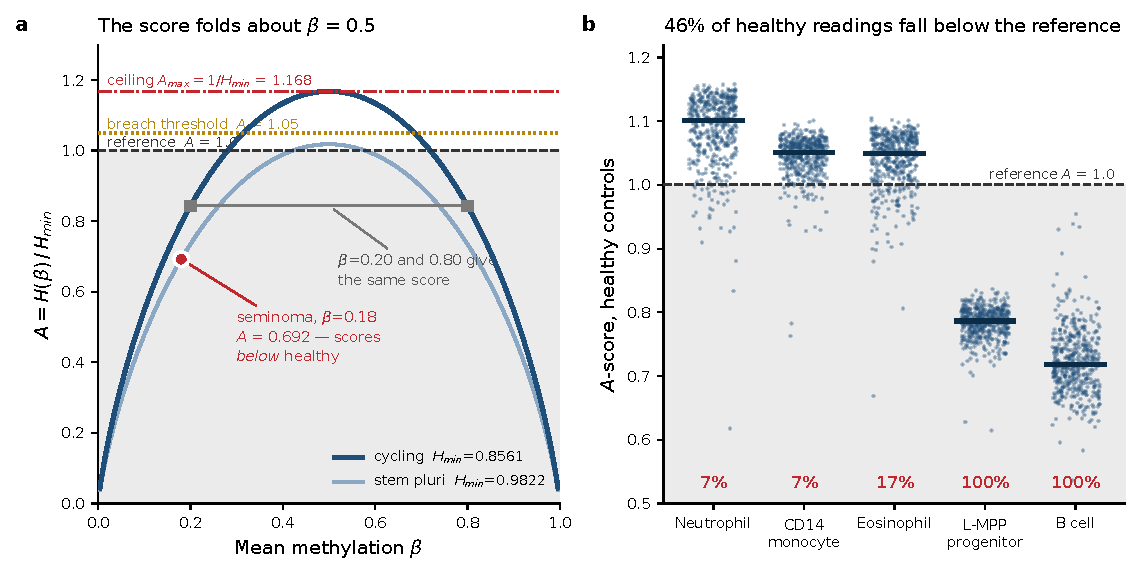
\includegraphics[width=0.94\textwidth]{fig4_ascore.pdf}
\caption{\textbf{(a)}~The A-score $A = H(\beta)/H_{min}$ is two-to-one in $\beta$: the binary entropy $H$ is symmetric about $0.5$, so $\beta = 0.20$ and $\beta = 0.80$ score identically and $dA/d\beta$ changes sign at the midpoint. The seminoma case ($\beta = 0.18$ on \texttt{stem\_pluri}, $A = 0.692$) is a strongly hypomethylated tumour that therefore scores \emph{below} the healthy reference; it is a passing regression test in \texttt{methylation report\_derivation\_tests.py}, making this a characterised domain restriction rather than an unrecognised defect. The structural ceiling $A_{max} = 1/H_{min}$ is also shown. \textbf{(b)}~A-scores for healthy controls only, AIBL cohort ($n = 471$ healthy of 726 total, five immune cell types). Pooled, $46.3\%$ of healthy readings fall below $A = 1.0$; for L-MPP progenitors and B cells, every healthy control does. This is the principal argument in Section~9 for calling $H_{min}$ a calibrated reference level rather than a physical floor.}
\label{fig:ascore}
\end{figure}


\textbf{Encoding surface:} nuclear chromatin accessible to DNMT1 maintenance machinery. \textbf{Irreversible event:} DNMT1-mediated maintenance methylation of a hemimethylated CpG. \textbf{Temperature:} \texttt{T\_body = 310.15 K} (isothermal --- no temperature sweep available in vivo).


\begin{lstlisting}
    e_bit    = k_B T_body ln2            = 2.9681 × 10⁻²¹ J per maintenance event
    N_CpG    = 19.6 × 10⁶
    E_floor  = N_CpG · e_bit             = 5.8175 × 10⁻¹⁴ J per division  ≈ 10⁶ ATP
\end{lstlisting}


\textbf{Metabolic coupling exponent} (the isothermal analogue of \texttt{n}):


\begin{lstlisting}
    M = ΔG_ATP / (R T_body) = 54,000 / (8.314462 × 310.15) = 20.94
\end{lstlisting}


the ratio of free energy per ATP hydrolysis to thermal energy at body temperature --- the biological counterpart of \texttt{$\hbar\omega$\_q/k\_B T}. It measures how strongly epigenomic fidelity responds to ATP/ADP perturbation, not temperature.


\textbf{The A-score.} With \texttt{H($\beta$) = -$\beta$ log$_{2}\beta$ - (1-$\beta$) log$_{2}$(1-$\beta$)} the binary entropy of mean methylation:


\begin{lstlisting}
    A = H(β) / H_min(class)
\end{lstlisting}


Tier structure: \texttt{A $\approx$ 1.00} at floor, healthy range; \texttt{A > 1.05} floor departure (detection threshold); \texttt{A > 1.10} floor breach --- architecture-class identity not maintainable.


\textbf{Global floor:} \texttt{H\_min\textasciicircum{}global = H(0.782) = 0.756500}, from Roadmap E073 frontal-cortex neuron.


\textbf{Temperature scaling} (cross-species, not human): \texttt{H\_min(T) = H\_min(37 $^{\circ}$C)$\cdot$(T\_body/310.15)\textasciicircum{}$\alpha$} with \texttt{$\alpha$ = 2.0}; 41\% cross-class variance reduction across n = 43 vertebrate species, r = -0.90.


\textbf{Per-class \texttt{H\_min}, five substrates} (G-002 + G-003b MCMC posteriors). Columns: methylation $\beta$, nucleosome occupancy, nucleosome fuzziness, windowed protection score, DELFI fragment size.


\begin{small}
\begingroup\footnotesize
\begin{tabularx}{\linewidth}{L{0.20\linewidth}YYYYY}
\toprule
\textbf{class} & \textbf{methyl} & \textbf{nucl} & \textbf{fuzz} & \textbf{wps} & \textbf{frag} \\
\midrule
cycling & 0.856055 & 0.980072 & 0.819030 & 0.627429 & 0.687936 \\
secretory & 0.843264 & 0.982560 & 0.847947 & 0.634534 & 0.697718 \\
immune & 0.838889 & 0.989930 & 0.830377 & 0.589644 & 0.711534 \\
terminal & 0.772837 & 0.992027 & 0.736973 & 0.958909 & 0.624938 \\
stromal & 0.862950 & 0.985667 & 0.832386 & 0.612686 & 0.724691 \\
stem\_pluri & 0.982166 & 0.799818 & 0.962920 & 0.905004 & 0.973583 \\
stem\_adult & 0.873718 & 0.960866 & 0.980754 & 0.988964 & 0.841327 \\
progenitor & 0.852216 & 0.972790 & 0.961900 & 0.988046 & 0.808978 \\
\bottomrule
\end{tabularx}
\endgroup
\end{small}


Methylation-substrate posterior widths \texttt{$\sigma$(H\_min)}: cycling 0.000800, secretory 0.000600, immune 0.001200, terminal 0.001100, stromal 0.001400, stem\_pluri 0.001800, stem\_adult 0.001600, progenitor 0.001700. Other-substrate CI half-widths: nucl 0.008427, fuzz 0.007359, wps 0.005649, frag 0.006878.


\textbf{Substrate AUCs and sources:} methylation 0.8663 (MESA 2024, Li et al. \textit{Genome Med}); nucleosome occupancy 0.852 (Doebley 2022; Corces 2018); fuzziness 0.779 (Esfahani 2022); WPS 0.761 (Snyder 2016); DELFI fragment size 0.940 (Cristiano 2019; Mathios 2022). Inter-substrate correlation r = 0.54.


\textbf{Calibration procedure (G-002).} 37 published reference cell measurements across 8 architecture classes, from ENCODE, Roadmap Epigenomics, and Lister et al.; senescent and cancer cells excluded. Likelihood:


\begin{lstlisting}
    ln L = −½ Σᵢ₌₁³⁷ ( [H(βᵢ)/H_min^{c(i)} − 1.0] / σ_A )²,     σ_A = 0.020
\end{lstlisting}


uniform prior \texttt{H\_min $\in$ [0.60, 1.00]}. Independently reproduced: 5 chains $\times$ 32 walkers $\times$ 5,000 production steps after 500 burn-in = 800,000 samples, max R-hat 1.00052, posterior means matching the published table to 3--4 decimal places.


\textbf{A closed form exists.} Differentiating the likelihood gives the maximum-likelihood solution


\begin{lstlisting}
    H_min(class) = Σ H(βᵢ)² / Σ H(βᵢ)        (sum over that class's reference cells)
\end{lstlisting}


a weighted mean of the class's reference-cell entropies, agreeing with the 800,000-sample chain to three decimal places (max deviation 7.6 $\times$ $10^{-4}$, on stem\_pluri). The MCMC and the one-line formula compute the same thing. \textbf{This is worth disclosing rather than protecting: it makes the entire calibration layer verifiable by a referee in five minutes.}


\textbf{The IAMAtlas.} 483,092 CpGs $\times$ 264 columns --- \texttt{cpg\_id}, \texttt{n\_classes\_with\_data}, 8 classes $\times$ 4 statistics, 115 cell types $\times$ 2 statistics. Per-CpG per-class credible intervals ship in \texttt{iamatlas\_v0\_1\_<class>\_brightness.csv} (\texttt{cpg\_id, class, mean, sd, ci\_lo, ci\_hi}). Class composition: immune 51, cycling 19, secretory 18, progenitor 11, terminal 9, stromal 5, stem\_adult 1, stem\_pluri 1. SHA-256 \texttt{41b7c16f043bce96e085a2b8b4e709efd2b862af9de8dbe9a8646e9fb94c32ee}.


\textbf{The flatness lesson --- methodologically the strongest work in the corpus.} The original Atlas build reported R-hat $\approx$ 1.01, ESS in the hundreds, zero divergences, and was \textit{wrong}: an identifiability ridge between \texttt{sigma\_class\_logit} and \texttt{log\_kappa} drove $\sigma$ $\rightarrow$ 0 and collapsed every cell type in a class onto the class mean. Clean convergence to a flattened posterior. The author caught it by comparing two cell types within a class --- a check no standard diagnostic performs --- and recorded the rule: \textit{a collapsed posterior is trivially easy to converge to.} After the fix, a distinctness test on terminal / progenitor / stromal / secretory finds 0 of 177 testable pairs below the 0.005 collapse signature; secretory reproduces at median 0.114 against a published 0.115.


\textbf{Disclosed limitation of the Atlas fit.} The fixed model is \texttt{mu\_logit \textasciitilde{} Normal(mu\_class\_logit, $\sigma$ = 3.0)} with shape equal to the number of observed (CpG, cell-type) pairs. Observations per pair are 1.00 in seven of eight classes --- one nearly unconstrained parameter per observation, so the model interpolates rather than pools, and the posterior-predictive checks (Pearson 0.999--1.000, MAE $10^{-4}$) are close to tautological. Stromal is the exception at 1.52 obs/pair, and its honest numbers --- Pearson 0.9341, MAE 0.0778 --- are the ones that carry information about fit quality. Accordingly the Atlas is best described as \textbf{a harmonised multi-atlas reference compilation with per-source precision}, not a hierarchical meta-analysis. Also: \texttt{rhat\_max} is a maximum over \textasciitilde{}5 $\times$ $10^{6}$ parameters, where multiplicity alone puts the max near 2--3 even under excellent mixing; the informative summary is the \textit{distribution} (fraction below 1.01 and 1.1, plus the 99th percentile).


\textbf{Empirical results, independently recomputed from the author's per-sample files:}


\begin{small}
\begin{tabularx}{\linewidth}{L{0.30\linewidth}YY}
\toprule
\textbf{test} & \textbf{reported} & \textbf{recomputed} \\
\midrule
GIFT AD vs HC (Mahalanobis) & d = +0.68 & d = +0.681, MWU p = 6.5 $\times$ $10^{-4}$ \\
GIFT PSP/CBD vs HC & d = -0.38 & d = -0.380, MWU p = 2.3 $\times$ $10^{-6}$ \\
AIBL AD vs HC & d = +0.20 & d = +0.200 \\
AIBL eosinophil A-score & d = -0.426 & d = -0.4255 \\
\bottomrule
\end{tabularx}
\end{small}


Pre-diagnostic breast signal: d = 1.88 and 2.10 in two EPIC-Italy cohorts, blood drawn >10 years before clinical diagnosis. TCGA: 27/28 cancer types show \texttt{A\_tumor > A\_normal}, 4,304 matched pairs, threshold fixed from healthy-cell calibration before cancer data was examined.







\section{The structural identity --- and the gap the author himself identifies}

The \texttt{floor\_breach} derivation states the cross-scale claim in its strongest honest form:


\begin{small}
\begin{tabularx}{\linewidth}{L{0.30\linewidth}YY}
\toprule
\textbf{} & \textbf{black hole} & \textbf{cancer cell} \\
\midrule
encoding surface & Bekenstein--Hawking horizon & chromatin / DNMT1 maintenance surface \\
temperature & \texttt{T\_\allowbreak{}H = $\hbar$c$^{3}$/\allowbreak{}8$\pi$GMk\_\allowbreak{}B} & \texttt{T\_\allowbreak{}body = 310.15 K} \\
bit count & \texttt{A\_\allowbreak{}horizon/\allowbreak{}4$\ell$\_\allowbreak{}P$^{2}$} & \texttt{N\_\allowbreak{}CpG = 19.6 $\times$ $10^{6}$} \\
cost per bit & \texttt{k\_\allowbreak{}B T\_\allowbreak{}H ln2} & \texttt{2.97 $\times$ $10^{-21}$ J} \\
floor metric & \texttt{S\_\allowbreak{}BH = A/\allowbreak{}4$\ell$\_\allowbreak{}P$^{2}$} & \texttt{H\_\allowbreak{}min(class)} \\
breach condition & \texttt{dS\_\allowbreak{}local/\allowbreak{}dt $\geq$ dS\_\allowbreak{}BH/\allowbreak{}dt} & \texttt{A = H($\beta$)/\allowbreak{}H\_\allowbreak{}min > 1.05} \\
breach event & horizon formation & malignant transformation \\
\bottomrule
\end{tabularx}
\end{small}


And then, in the paper's own words:


> \textit{The open problem is the quantitative bridge: showing that the specific value of \texttt{H\_min} for a > given architecture class can be derived from first principles through the full > Landauer--Jacobson--IAM chain without reference to empirical calibration. That derivation would > complete the unification.}


> \textit{The structural derivation presented here is complete and publishable. The full numerical > unification \ldots{} is the open problem that would make this a complete theory rather than a > structural result.}


This is the correct self-assessment and it is stated in the author's own preprint. \textbf{What is established is a template; what is open is the numerical bridge.} A reader should evaluate the framework on that basis rather than on the stronger claim that appears in some summary material.


\textbf{Why the bridge is hard, stated concretely.} In the transmon case \texttt{$\Delta$\_Al} does double duty: it sets the bath temperature (\texttt{T\_gap = $\Delta$\_Al/k\_B}) \textit{and} it is the energy quantum of the observable (one quasiparticle costs \texttt{$\Delta$\_Al}). That is why \texttt{E\_erase/$\Delta$\_Al = ln2} yields a countable number and \texttt{x\_qp} emerges parameter-free. In the cellular case no single energy plays both roles: \texttt{T\_body} fixes \texttt{e\_bit} as an energy, while the observable \texttt{H\_min} is an entropy in bits. The chain therefore has no surface quantum to divide by, which is precisely why \texttt{H\_min} is calibrated. The two missing entries in the cellular column of the author's own structural table are an \textbf{explicit event rate} (the analogue of \texttt{$\tau$\_TLS-$^{1}$}; currently listed as ``implicit in the DNMT1 maintenance cycle``) and a \textbf{participation volume} (the analogue of \texttt{$\pi\lambda$\_L$^{3}$}). Supplying both would close the bridge.







\section{The honest ledger --- derived, calibrated, or fitted}

The single most useful table for a referee, and supplied deliberately.


\begin{small}
\begin{tabularx}{\linewidth}{L{0.30\linewidth}YY}
\toprule
\textbf{quantity} & \textbf{status} & \textbf{notes} \\
\midrule
\texttt{E\_\allowbreak{}bit = k\_\allowbreak{}B T ln2} & \textbf{established} & Landauer \\
\texttt{1/\allowbreak{}4 = 2$\pi$/\allowbreak{}8$\pi$} & \textbf{exhibited} & ratio shown; independent derivation is the open point \\
\texttt{$\beta$\_\allowbreak{}m = $\Omega$\_\allowbreak{}m/\allowbreak{}2} & \textbf{derived}, given measured \texttt{$\Omega$\_\allowbreak{}m} & virial 1/2 is exact for 1/r \\
\texttt{E(a) = exp(1-1/\allowbreak{}a)} & \textbf{derived} from horizon thermodynamics & functional form, not fitted \\
\texttt{$\mu$(z=0) = 0.8639} & \textbf{derived} from \texttt{$\beta$\_\allowbreak{}m} & no freedom once \texttt{$\beta$\_\allowbreak{}m} fixed \\
\texttt{$\Sigma$ $\equiv$ 1} & \textbf{derived} (null geodesics) & imposed in the MGCAMB runs \\
\texttt{T\_\allowbreak{}gap = $\Delta$\_\allowbreak{}Al/\allowbreak{}k\_\allowbreak{}B} & \textbf{derived} & BCS \\
\texttt{V\_\allowbreak{}eff = $\pi\lambda$\_\allowbreak{}L$^{3}$} & \textbf{derived} & London Green's function, O(1) geometric factor \\
\texttt{x\_\allowbreak{}qp\textasciicircum{}min} & \textbf{predicted}, parameter-free & sensitive to \texttt{$\tau$\_\allowbreak{}TLS} within published range \\
\texttt{M} (semiconductor) & \textbf{computed} from datasheets & no free parameter \\
\texttt{M = $\Delta$G\_\allowbreak{}ATP/\allowbreak{}RT = 20.94} & \textbf{computed} from published \texttt{$\Delta$G\_\allowbreak{}ATP} & a constant, not a per-patient reading \\
\texttt{$\alpha$ = 2.0} (temperature) & \textbf{fitted} & cited \texttt{E\_\allowbreak{}a} 40--80 kJ/mol maps to $\alpha$ 1.2--2.4, so consistent with rather than predictive of 2.0 \\
\texttt{t\_\allowbreak{}max} (DunedinPACE) & \textbf{fitted} & stated as the single free parameter in that section \\
\texttt{f\_\allowbreak{}geom = $\Omega$\_\allowbreak{}m/\allowbreak{}2$\pi$} (M--$\sigma$) & \textbf{one identification} & acknowledged in the paper \\
\texttt{$\eta$, $\sigma^{2}$/\allowbreak{}c$^{2}$} (M--$\sigma$) & \textbf{normalizations} & adjusted to the observed scale \\
\textbf{\texttt{H\_\allowbreak{}min(class)}} & \textbf{calibrated} & MCMC posterior over 37 healthy reference cells; closed form = weighted mean of their entropies \\
\texttt{A > 1.05} threshold & \textbf{derived from \texttt{H\_\allowbreak{}min} + \texttt{$\sigma$\_\allowbreak{}A}} & fixed before cancer data examined \\
\texttt{m\_\allowbreak{}e} fixed point & \textbf{predicted}, 6.6 ppm & \texttt{(2$\pi$)\textasciicircum{}(-2/\allowbreak{}5)} of the prefactor is derived (via \texttt{T\_\allowbreak{}GH}); only the residual \texttt{(2$\pi$)\textasciicircum{}(3/\allowbreak{}10)} is not. \texttt{m\_\allowbreak{}e $\propto$ H$_{0}$\textasciicircum{}(2/\allowbreak{}5)} does \textbf{not} imply drift --- \S6 \\
\texttt{P\_\allowbreak{}SB = P\_\allowbreak{}Hawking} & \textbf{exact identity}, 12 sig figs & Stefan--Boltzmann on the horizon vs Hawking luminosity \\
\texttt{M\_\allowbreak{}lens/\allowbreak{}M\_\allowbreak{}dyn = 1/\allowbreak{}$\mu$(z)} & \textbf{predicted}, 15.7\% at z=0 & follows from \texttt{$\mu$(z)}; no new parameter \\
Barrow \texttt{$\Delta$}, Tsallis \texttt{$\delta$} & \textbf{fitted} in those frameworks & IAM's \texttt{$\beta$\_\allowbreak{}m} is not --- this is the positioning argument \\
\bottomrule
\end{tabularx}
\end{small}


\textbf{On ``zero free parameters.``} The defensible statement is narrower than the one in several abstracts, and it is still strong: \textbf{no parameter is fitted to the data the framework is tested against.} \texttt{H\_min} is calibrated on healthy reference cells only and frozen before any disease data is seen; \texttt{$\beta$\_m} comes from \texttt{$\Omega$\_m}; the cancer-direction test and the $\mu_{0}$ chains introduce nothing. That is a real and unusual methodological virtue. ``Zero free parameters`` full stop is not accurate once \texttt{$\alpha$}, \texttt{t\_max}, \texttt{f\_geom}, and the platform \texttt{n} are counted, and a referee will count them.







\section{What would falsify IAM}

On the record before the data:


\begin{enumerate}\setlength\itemsep{2pt}
  \item \textbf{Euclid DR1 (Oct 2026)} --- \texttt{$\mu_{0}$ = -0.136}, \texttt{$\Sigma$ = 1}, scale-independent, at projected 3.4$\sigma$. A measurement of \texttt{$\mu_{0}$ = 0 $\pm$ 0.04} falsifies the cosmological sector.
  \item \textbf{Cluster lensing-to-dynamical mass ratio} --- \texttt{M\_lens/M\_dyn = 1/$\mu$(z)}, predicting a **15.7\% discrepancy at z = 0**, testable now on eROSITA and Euclid cluster samples. Independent of the \texttt{$\mu_{0}$} chain constraint and available on a shorter timescale.
  \item \textbf{Single-device \texttt{x\_qp} invariant} --- \texttt{x\_qp $\cdot$ n\_cp $\cdot$ $\tau$\_TLS $\cdot$ $\pi\lambda$\_L$^{3}$ / $\tau$\_qp = ln2} with \texttt{$\tau$\_TLS} measured on the same device. A significant departure from 0.693 falsifies the quantum sector.
  \item \textbf{\texttt{$\sigma$\_crit $\approx$ 4 km s-$^{1}$}} --- the minimum halo velocity dispersion below which the virial partition cannot close and no satellite virializes. Directly checkable against Milky Way satellite dispersion catalogues; a confirmed virialized halo well below 4 km/s falsifies it.
  \item \textbf{DESI DR2 \texttt{w$_{0}$--w\_a}} --- \texttt{w\_info(a) = -1 - 1/(3a)}, zero free parameters, mildly phantom and asymptoting to -1.
  \item \textbf{Cluster-merger lensing offsets} --- a \textit{null} prediction: with \texttt{$\Sigma$ = 1} and unmodified light deflection, lensing-peak/gas offsets must follow $\Lambda$CDM collisionless dynamics. A detected deviation falsifies the sector split.
  \item \textbf{Gravitational decoherence temperature scaling} --- \texttt{$\tau$ $\propto$ T$^{2}$}, giving 16$\times$ longer coherence between 10 and 40 mK where Penrose--Di\'osi predicts no change. Feasible now for \texttt{m > $10^{-12}$} kg.
  \item \textbf{Gravitational decoherence profile shape} --- rate zero at \texttt{t = 0} rather than maximal; discrimination peaks at \texttt{$\eta$ = 0.23} with \texttt{$\Delta$P = 0.139}. 5$\sigma$ at \texttt{m > 3.65 $\times$ $10^{-15}$} kg.
  \item \textbf{\texttt{r\_core $\propto$ $\sigma^{2}$}} --- dark-matter core radius against dwarf-galaxy rotation curves. The scaling is the prediction; the normalization is open (see \S4.5).
  \item \textbf{DNMT1 single-molecule fidelity across 15--42 $^{\circ}$C} --- predicted \texttt{(T$_{2}$/T$_{1}$)\textasciicircum{}-2}. Requires a kinetics collaborator, no patients, no grant. **This is the cleanest available test of whether the cellular floor is thermodynamic rather than statistical**, and no other model predicts it.
  \item \textbf{Prospective cellular validation} --- Sister Study, UK Biobank (n = 55,746 incident cancers).
\end{enumerate}







\section{Executable verification suites}

A test suite for the cellular derivations ships with the framework and was \textbf{run here}, not merely read:


\begin{small}
\begin{tabularx}{\linewidth}{L{0.30\linewidth}Y}
\toprule
\textbf{suite} & \textbf{result} \\
\midrule
\texttt{methylation report\_\allowbreak{}derivation\_\allowbreak{}tests.py} & \textbf{12/12 pass} \\
\bottomrule
\end{tabularx}
\end{small}


Selected checks, with values as emitted: \texttt{H\_min\textasciicircum{}global = H(0.782) = 0.756499}; A-score \texttt{H(0.685)/0.856055 = 1.0500}; Landauer denominator at 75 $^{\circ}$C \texttt{= 3.332 $\times$ $10^{-21}$ J}.


Several tests state candidly that an identity holds \textbf{by construction}, which correctly distinguishes an internal consistency check from an empirical validation.


The suite establishes internal self-consistency and reproduction of published reference values. It does not, and does not claim to, test the framework against nature.





\section{Provenance, reproducibility, and known weaknesses}

\textbf{Validation discipline.} Every VAL block carries \texttt{PREREG.md} written before execution and a sealed \texttt{OUTCOME.md}; declared null suites; label-permutation tests; amendments disclosed \textit{after} the observable was seen with explicit second-best-path notation; per-run \texttt{cohort\_manifest.json}; SHA-256 atlas tracking. Outcomes are permitted to return RESTATE or FAIL and several do --- VAL-004's bimodality direction reversed, VAL-006's chr6 signal died under look-elsewhere correction, VAL-128 failed opposite to pre-registration. These are recorded, not removed.


\textbf{Weaknesses the author flags, or that are flagged here:}


\begin{itemize}\setlength\itemsep{2pt}
  \item \texttt{H\_min} is a calibration, not a derivation (\S5) --- the author's own stated open problem.
  \item \texttt{A = H($\beta$)/H\_min} is \textbf{two-to-one in $\beta$}: \texttt{H} is symmetric about 0.5, so $\beta$ = 0.20 and $\beta$ = 0.80 both give A = 0.8433 at the cycling floor, and \texttt{dA/d$\beta$} changes sign at $\beta$ = 0.5. This generates direction flips in cohorts whose mean $\beta$ approaches 0.5 and is the mechanism behind several recorded \texttt{LE\_DIRECTION\_FLIP} outcomes. **This is a known and characterised property, not an unrecognised bug** --- \texttt{methylation report\_derivation\_tests.py} Test 12 is a passing regression test for it under the name \textit{seminoma inversion}, using the real clinical case of a strongly hypomethylated germ-cell tumour ($\beta$ = 0.18 on \texttt{stem\_pluri}), which scores A = 0.6924 and therefore reads as \textit{below} the healthy reference. It should be stated as a documented domain restriction of the instrument --- valid for $\beta$ above 0.5, inverting below --- rather than left for a reader to find.
  \item Related and also tested: the score has a structural ceiling \texttt{A\_max = 1/H\_min} (1.1681 for cycling methylation, confirmed by Test 6). For \texttt{stem\_pluri} the ceiling on the methylation, fuzziness and fragment substrates lies \textit{below} the breach threshold (Test 7), so those substrates structurally cannot register a breach for pluripotent cells. The runtime handles this with a saturation flag and an \texttt{A\_active} score that excludes saturated substrates (Tests 8, 10) --- a sound mitigation that belongs in the methods section of any paper using it.
  \item \textbf{Roughly half of the author's own healthy-control readings fall below A = 1.0} (48.4\% of all readings, 46.3\% of healthy controls, in the AIBL per-cell-type data; L-MPP and B cells are 100\% below; minimum observed A = 0.5357). A floor that healthy cells sit beneath is functioning as a normalisation constant rather than a physical bound. This is the sharpest internal tension in the framework and is unresolved.
  \item The Mahalanobis ``negative direction`` result for PSP/CBD is a \textbf{dispersion} difference, not a signed direction: Mahalanobis distance is non-negative by construction (observed range 13.41--80.44), so \texttt{d = -0.38} means PSP samples cluster more tightly about the healthy centroid than healthy controls do. It should be tested with Levene/Bartlett, not Cohen's \texttt{d} on distances. 115 dimensions estimated from 193 controls is also under-determined.
  \item Preclinical effect sizes sit near array noise: \texttt{$\Delta$A = +0.014} corresponds to \texttt{$\Delta\beta$ $\approx$ -0.009}, roughly one third of 450K/EPIC technical CV. The plate-position null was \textbf{skipped} because plate metadata is absent from the GEO series matrices; sentrix ID and position are recoverable from raw IDATs and this test is outstanding.
  \item The cosmology is a \textbf{null constraint}, not a detection (\S3.2).
  \item Consistency of the dual-sector split --- distances on \texttt{H\_phot}, growth on \texttt{H\_matt} --- is the standard first objection: applied naively it is not derived from an action and would generically violate \texttt{$\nabla$\_$\mu$ T\textasciicircum{}$\mu\nu$ = 0}. \textbf{\texttt{IAM\_BH\_Thermodynamics} addresses this}, formulating the informational term as a covariant scalar functional that vanishes in exact stationary spacetimes and claiming preservation of the Bianchi identity with no additional propagating degrees of freedom. **\texttt{IAM\_Lensing\_Dynamics} and \texttt{3Way\_Mass\_Discrepancy} answer it a second, more direct way**, showing the linearized Einstein equations for the metric potentials are unmodified, that no anisotropic stress or extra perturbative degree of freedom is introduced, and that the Weyl-potential relation is preserved. So the objection is addressed in three places --- and cited in none of them from \texttt{Dual\_Sector\_Perturbation\_Cosmology}, which is the paper a referee will read first. These claims still need independent checking, but the fix to the \textit{presentation} is free: cross-reference them.
  \item \texttt{$\beta$\_m = $\Omega$\_m/2} uses the present-day \texttt{$\Omega$\_m}, which evolves, so the coupling is epoch-specific as written. An expression in terms of a time-invariant quantity, or an explicit argument for why the present epoch is privileged, is needed. Note the framework's own \texttt{E(1)/e $\approx$ 36.8\%} result --- the present epoch sitting at the activation function's inflection --- may be the beginning of that argument.
  \item In the electron-mass paper the residual \texttt{(2$\pi$)\textasciicircum{}(3/10)} factor has a proposed geometric origin but no completed derivation (the paper's own Open Problem 1), so ``zero free parameters`` is not yet supported by that chain. The companion gap is that \texttt{$\mu$ = m\_p/m\_e} involves the proton, and the paper states that composite particles --- not fundamental decoherence loops in the IAM sense --- are not treated. \textit{Note: the \texttt{m\_e $\propto$ H$_{0}$\textasciicircum{}(2/5)} scaling does} \textbf{not} *imply a varying electron mass; \S6 resolves that explicitly, the fixed point being evaluated at the present-epoch projector with \texttt{H$_{0}$} entering as a constant. Do not let a reader assume otherwise.*
  \item \textbf{Two inequivalent A-score definitions circulate in the methylation report documents.} The operative one, used in all numerical results, is \texttt{A = H($\beta$)/H\_min(class)} --- verified: `H(0.740)/0.856055 = 0.9658\texttt{ and }H(0.580)/0.856055 = 1.1465`, matching the published healthy and tumour class means of 0.96576 and 1.14648. But a three-component decomposition elsewhere defines \texttt{A = 1 + C$_{3}$/H\_actual} with \texttt{C$_{3}$ = max(0, H\_actual - H\_min)}, which equals \texttt{2 - H\_min/H\_actual}. The two agree only at \texttt{A = 1} and diverge away from it. One definition must be retired before submission.
  \item \textbf{The chain count is well defined; the convergence claim attached to it is not.} The root README's accounting is explicit and checks out --- *17 converged MCMC chains (12 Level 1 via MGCAMB + 5 Level 2 via modified CAMB)*, plus a baryon-asymmetry chain as ``Test 18,`` giving the 18 independent tests. The 18 \texttt{.progress} files in the repository match that breakdown exactly. What does \textbf{not} hold is \texttt{mgcamb\_validation/README.md} line 120: *``All 12 runs converged with R-1 < 0.01.``* Read at their final iterations, ten of the twelve Level-1 runs are below 0.01, but \texttt{iam\_fixed\_mu0} (0.022565) and \texttt{iam\_float\_mu0} (0.024170) --- the two Planck-alone IAM runs --- are not. On the Level-2 side four of five are below 0.01 and \texttt{iam\_l2b\_runA} sits at exactly 0.010000. So the defensible statement is **14 of 17 production chains strictly below threshold, one at threshold, two marginal at $\approx$0.023**, with the baryon chain converged at 0.009907. Either extend those two runs or restate the claim; chain bookkeeping is the first thing a cosmology referee audits, and this one is checkable in a single command.
  \item The \texttt{H\_min} values have a \textbf{revision history} that should be stated rather than discovered: immune/haematopoietic moved from a calibration value of 0.795000 to the current 0.8389 $\pm$ 0.0012 after MCMC reanalysis of six immune cell types, revising immune A-scores downward by 0.055. Publishing the frozen-value provenance and date is what makes ``frozen before disease testing`` checkable.
  \item The $\Lambda$ ratio is \texttt{($\ell$\_P/$\ell$\_H)$^{2}$ $\times$ 0.0824}; the bare ratio supplies all 122 orders and \texttt{$\ell$\_H = c/H$_{0}$} uses the measured \texttt{H$_{0}$}.
\end{itemize}







\section{Recommended reading order for a physicist}

\begin{enumerate}\setlength\itemsep{2pt}
  \item \textbf{\texttt{xqp\_.tex}} --- the residual quasiparticle floor. Self-contained, parameter-free, explains a standing anomaly, single-device falsifiable invariant. Requires no commitment to anything else.
  \item \textbf{\texttt{Baryon\_Asymmetry\_as\_a\_Derived\_Quantity}} --- \texttt{$\eta$} from the CMB with the BBN prior removed. Subtractive, 0.36\%.
  \item \textbf{\texttt{Bekenstein\_coefficient}} --- the geometric origin of 1/4. The conceptual core of P3.
  \item \textbf{\texttt{Dual\_Sector\_Perturbation\_Cosmology\_CAMB}} + the chains --- the implementation and its honest null result.
  \item \textbf{\texttt{floor\_breach\_derivation}} --- the cross-scale structural claim \textit{and} the author's own statement of what remains open.
  \item \textbf{\texttt{Mahaffey\_2026\_cell\_thermodynamics}} --- the cellular application, read with \S4 and \S8 in hand.
\end{enumerate}







\section{Errata in the existing preprints --- disclosed}

\begin{enumerate}\setlength\itemsep{2pt}
  \item \textbf{Bekenstein--Hawking entropy formula.} \texttt{IAM\_M\_Sigma} and the Hubble2Methyl document write \texttt{S\_BH = 4$\pi$GM$^{2}$/($\hbar$c$^{3}$)}. The correct expression is \texttt{4$\pi$GM$^{2}$/($\hbar$c)}; the published form is low by exactly \texttt{1/c$^{2}$} (verified: ratio 1.1127 $\times$ $10^{-17}$ for a 10 M$_{\odot}$ black hole).
  \item \textbf{\texttt{ln2} double-counted in the Landauer identity.} The bit count is \texttt{N = S/(k\_B ln2)}, so \texttt{N k\_B T ln2 = T S} and the \texttt{ln2} cancels. Verified numerically: \texttt{k\_B T\_BH $\cdot$ S/k\_B = Mc$^{2}$/2} to ratio 1.0000000000. **The correct universal fraction is exactly 1/2 (50\%), not \texttt{ln2/2} (34.7\%).** This should also be attributed: \texttt{TS = Mc$^{2}$/2} for Schwarzschild is the Smarr formula (Bardeen--Carter--Hawking 1973).
  \item \textbf{\texttt{M--$\sigma$} exponent attribution.} The \texttt{$\sigma^{4}$} scaling enters by substituting the \textit{empirical} Faber--Jackson relation \texttt{M\_bulge $\propto$ $\sigma^{4}$} into \texttt{S\_BH $\propto$ M$^{2}$}; it is not fixed by the post-Newtonian order of gravitational radiation. Quadrupole GW luminosity scales as \texttt{(v/c)$^{5}$}, not the \texttt{(v/c)$^{2}$} used.
  \item \textbf{\texttt{n\_bio} presentation.} \texttt{The\_Cellular\_Margin} presents \texttt{n\_bio = 20.94} as a per-patient reading; it is a constant (\texttt{$\Delta$G\_ATP/RT}) and cannot vary with disease. The per-patient quantity is the A-score.
  \item \textbf{Landauer floor stated as \texttt{kT}} rather than \texttt{kT ln2} in the same clinician-facing document.
  \item \textbf{Cryogenic rationale.} Quantum computers are cooled to suppress thermal excitation and maintain superconductivity, not to lower Landauer erasure cost.
  \item \textbf{\texttt{n\_bio} and the Mahaffey number are one quantity.} Early the methylation report documents wrote the cellular ratio as \texttt{n\_bio}; it is \texttt{M = $\Delta$G\_ATP/(RT) = 20.94}. Drafts of this document and of \texttt{IAM\_Hubble2Methyl} (l.\,2192 in an earlier revision) put a \texttt{ln2} in the denominator and reported 30.21 for the cell and 117 for logic; the author's ruling (2026-09-19) defines \texttt{M} against \texttt{k\_B T} with no \texttt{ln2}, and every value in this document is now on that definition (cell 20.94; Apple M1 81; transmon 1 at \texttt{T\_gap}). Any remaining 117 or 30.21 elsewhere in the corpus is the withdrawn form.
  \item \textbf{\texttt{$\Delta\chi^{2}$} framing is self-contradictory within a single file.} \texttt{README.md} line 11 reports \texttt{$\Delta\chi^{2}$ = +0.54} best-fit versus $\Lambda$CDM; lines 464--466 of the \textit{same file} report a combined \texttt{$\Delta\chi^{2}$ = 79.8}, described as ``equivalent to 8.9$\sigma$`` (the text does flag it as a simplified analysis). The same table is repeated at \texttt{mgcamb\_validation/chains/README.md} lines 627--629. A referee who reads both concludes the headline number is chosen for effect. Adopt \texttt{+0.54} everywhere and retire the 79.8 framing, or separate them so unmistakably that no reader can take the larger number as the result of the MCMC analysis.
\end{enumerate}




\textit{Prepared as a reference summary. Section 4 and Section 8 are included at the author's instruction: the stated policy of this project is that weaknesses are disclosed by the author rather than discovered by the reader.}



\end{document}
